\documentclass[border=8pt]{standalone}
\usepackage{fontspec}
\setmainfont{TeX Gyre Heros}
\setsansfont{TeX Gyre Heros}
\usepackage{tikz}
\usetikzlibrary{arrows.meta,positioning,shapes.geometric,shapes.misc,shapes.symbols,fit,backgrounds,calc,chains}
\definecolor{ink}{HTML}{111827}
\definecolor{band}{HTML}{F3F4F6}
\definecolor{band2}{HTML}{E5E7EB}
\definecolor{accent}{HTML}{1D4ED8}
\definecolor{accentlight}{HTML}{DBEAFE}
\definecolor{warn}{HTML}{B91C1C}
\definecolor{warnlight}{HTML}{FEE2E2}
\definecolor{ok}{HTML}{047857}
\definecolor{oklight}{HTML}{D1FAE5}
\tikzset{
  >={Stealth[length=2.6mm]},
  box/.style={draw=ink, line width=0.6pt, rounded corners=9pt, fill=white, align=center,
              inner sep=4pt, font=\small},
  pill/.style={box, rounded corners=13pt},
  key/.style={box, fill=accentlight, draw=accent, line width=0.9pt},
  soft/.style={box, fill=band},
  dec/.style={draw=ink, line width=0.6pt, diamond, aspect=2.2, align=center, inner sep=1.5pt,
              font=\footnotesize, fill=white},
  arr/.style={->, draw=ink, line width=0.6pt},
  darr/.style={->, draw=ink, line width=0.6pt, dashed},
  lbl/.style={font=\footnotesize, fill=white, inner sep=1.5pt},
  layer/.style={draw=band2, fill=band, rounded corners=6pt},
  title/.style={font=\bfseries\small, align=left, anchor=west},
}
\begin{document}
\sffamily\hyphenpenalty=10000\exhyphenpenalty=10000

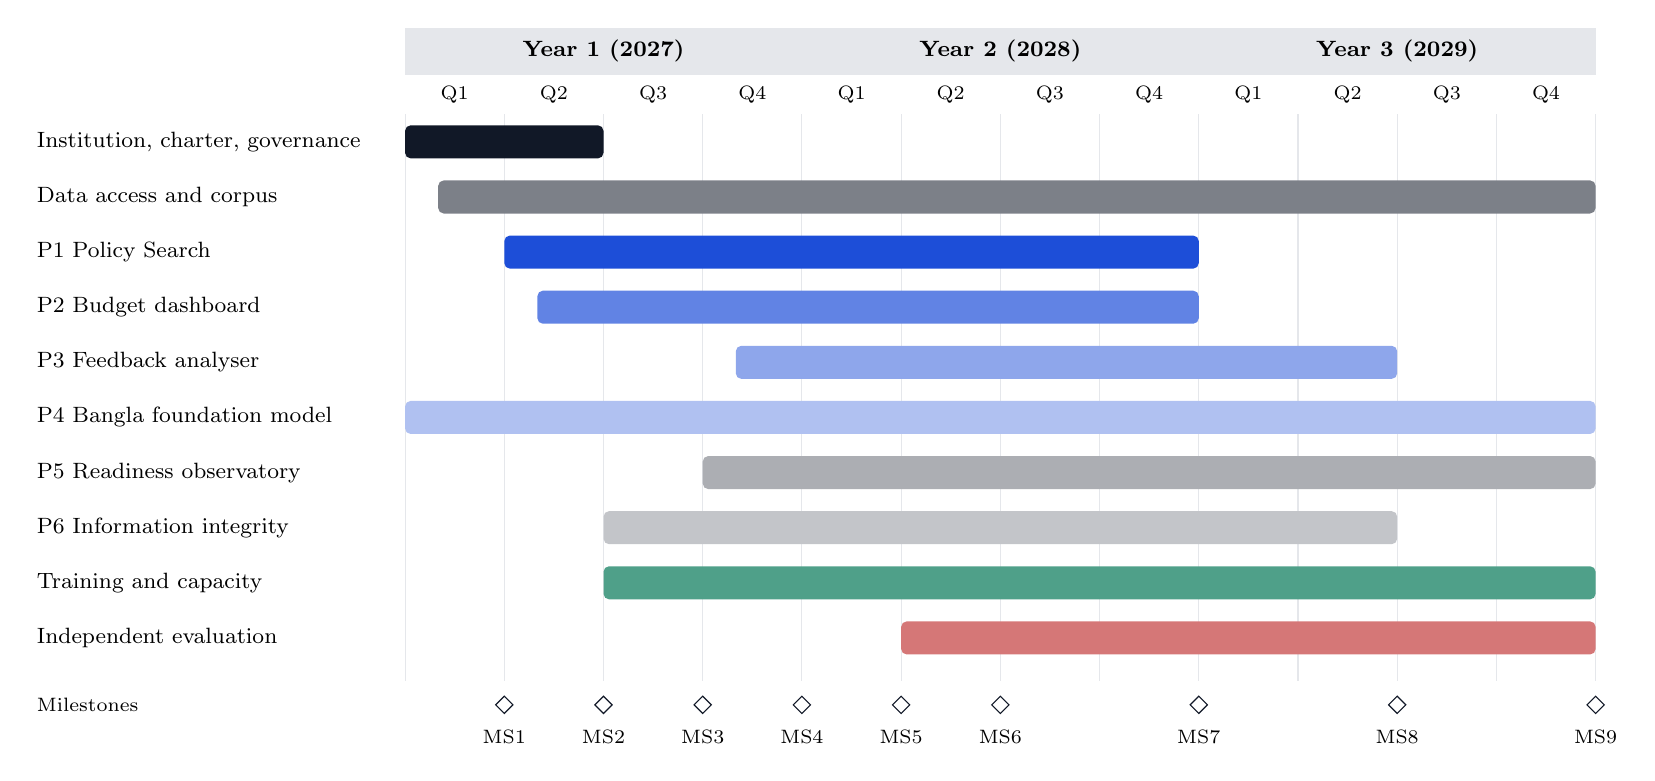
\begin{tikzpicture}
\def\x{4.2mm}  % per month
\def\h{7mm}    % per row
\def\L{48mm}   % label width
% header
\foreach \yr/\s in {Year 1 (2027)/0,Year 2 (2028)/12,Year 3 (2029)/24} {
  \fill[band2] (\L+\s*\x,0) rectangle (\L+\s*\x+12*\x,6mm);
  \node[font=\bfseries\footnotesize] at (\L+\s*\x+6*\x,3mm) {\yr};
}
\foreach \q in {0,...,11} {
  \pgfmathtruncatemacro{\qq}{mod(\q,4)+1}
  \node[font=\scriptsize] at (\L+\q*3*\x+1.5*\x,-2.5mm) {Q\qq};
}
\foreach \m in {0,3,...,36} \draw[band2, line width=0.4pt] (\L+\m*\x,-5mm) -- (\L+\m*\x,-5mm-10*\h-2mm);
% rows: label, start month (0-based), end month, style
\newcommand{\gbar}[5]{%
  \node[font=\footnotesize, anchor=west, text width=\L-2mm] at (0,-5mm-#1*\h-0.5*\h) {#2};
  \fill[#5, rounded corners=2pt] (\L+#3*\x,-5mm-#1*\h-0.2*\h) rectangle (\L+#4*\x,-5mm-#1*\h-0.8*\h);}
\gbar{0}{Institution, charter, governance}{0}{6}{ink}
\gbar{1}{Data access and corpus}{1}{36}{ink!55}
\gbar{2}{P1 Policy Search}{3}{24}{accent}
\gbar{3}{P2 Budget dashboard}{4}{24}{accent!70}
\gbar{4}{P3 Feedback analyser}{10}{30}{accent!50}
\gbar{5}{P4 Bangla foundation model}{0}{36}{accent!35}
\gbar{6}{P5 Readiness observatory}{9}{36}{ink!35}
\gbar{7}{P6 Information integrity}{6}{30}{ink!25}
\gbar{8}{Training and capacity}{6}{36}{ok!70}
\gbar{9}{Independent evaluation}{15}{36}{warn!60}
% milestones
\foreach \m/\n in {3/1,6/2,9/3,12/4,15/5,18/6,24/7,30/8,36/9} {
  \node[draw=ink, fill=white, diamond, inner sep=1.6pt] at (\L+\m*\x,-5mm-10*\h-5mm) {};
  \node[font=\scriptsize, anchor=north] at (\L+\m*\x,-5mm-10*\h-7mm) {MS\n};
}
\node[font=\scriptsize, anchor=west] at (0,-5mm-10*\h-5mm) {Milestones};
\end{tikzpicture}
\end{document}
